%\VignetteIndexEntry{Getting started with the package}
%\VignetteKeywords{getting started}
%\VignettePackage{synbreed}

\documentclass[a4paper,11pt]{article}
\usepackage{natbib}
\bibliographystyle{apalike}

% Preabmle parts
\usepackage[T1]{fontenc}
\usepackage{url}
\usepackage{hyperref}
\usepackage{times}

%PSTricks
\usepackage{pdftricks}
\begin{psinputs}
  \usepackage{pst-all}
\end{psinputs}

\usepackage{bm}
\usepackage{amsmath}
\usepackage{amssymb}
\usepackage{latexsym}
\usepackage{verbatim}
\usepackage{epsfig}
\usepackage{comment}
\usepackage{pdfpages}
%\usepackage{algorithm2e}
\usepackage{subfigure}

\usepackage{Sweave}
\usepackage{fancyvrb}
\definecolor{Sinput}{rgb}{0.56,0,0}
\DefineVerbatimEnvironment{Sinput}{Verbatim}{formatcom={\color{Sinput}},fontsize=\small,fontshape=sl}
\definecolor{Soutput}{rgb}{0,0,0.56}
\DefineVerbatimEnvironment{Soutput}{Verbatim}{formatcom={\color{Soutput}},fontsize=\small,fontshape=sl}

\newcommand{\Cov}{\text{Cov}}


\title{The R-Package 'synbreed'}
\author{
Valentin Wimmer\thanks{Author of correspondence. Contact: Institute for plant breeding, Technical University of Munich, Emil-Ramann-Str. 4,
	85354 Freising, Germany, Email: \texttt{Valentin.Wimmer@wzw.tum.de}}\\
} \date{\today}

\begin{document}
%%%%%%%%%%%%%%%%%%%%%%%%%%%%%%%%%%%%%%%%%%%%%%%%%%%%%%%%%%%%%%%%%%%%%%
% Sweave
%%%%%%%%%%%%%%%%%%%%%%%%%%%%%%%%%%%%%%%%%%%%%%%%%%%%%%%%%%%%%%%%%%%%%%
%Put all in another directory

 \setkeys{Gin}{width=0.9\textwidth}

%%%%%%%%%%%%%%%%%%%%%%%%%%%%%%%%%%%%%%%%%%%%%%%%%%%%%%%%%%%%%%%%%%%%%%
% Initial R code
%%%%%%%%%%%%%%%%%%%%%%%%%%%%%%%%%%%%%%%%%%%%%%%%%%%%%%%%%%%%%%%%%%%%%%




\maketitle


\begin{abstract}
  \noindent This document gives an introduction to the R-package
  'synbreed'. The package contains tools and methods for plant and animal breeding. The goal is to create an analysis pipeline for genomic selection. This comprises tools
  for genotypic, phenotypic and pedigree data. The steps of a typical analysis are presented in this document. This starts with the coding of the marker data, followed by the estimation of relatdness according
  to pedigree or molecular marker data, e.g. according to \citet{vanRaden2008}. Finally the estimation of breeding values and estimation of variance components using mixed models is described. 
  All steps are illustrated using simulated data for maize.\\

  \noindent{\bf Keywords:} synergistic plant and animal breeding, simulation, pedigree, genomic marker data, mixed models, genomic selection
  

  
\end{abstract}


\section{Introduction}\label{sec:Introduction}

The R-package 'synbreed' aims to provide the tools that are necessary to analyze data of breeding programs and estimate (genomic) breeding values. Of course,
there exists already software for this purpose. In R, package \texttt{genetics} contains classes and methods for handling genetic data \citep{Warnes2003} and package \texttt{qtl} could be used for QTL analysis in experimental crosses \citep{Broman2003}.  The idea of this package is to collect the methods in one package, so that analysis can be performed in one software with just a few steps as described in this document. 
Additional, this package takes care of special problems of modern breeding programs as the use of doubled haploid (DH) lines in plant breeding.  To our knowledge, there is no package in R which provides comparable features. Most of packages source code is written in R, so that methods could 
easily be adopted for own purposes. Package \texttt{synbreed} makes no stringent restriction concerning input data format to allow for a wide range of possible data sources.

Modern breeding programs use genomic information of individuals. On the genomic level, individuals could be distinguished by \textit{alleles} which are different states at a particular gene locus. In diploid species, every individuals has two sets of chromosomes and thus two copies of each allele at a locus. 
If both alleles are the same, the individual is homozygous for this locus, otherwise it heterozygous. For many species  \textit{molecular markers} are available and used to detect SNP (single nucleotide polymorphism) variation which occurs when a single nucleotide (\texttt{A}, \texttt{T}, \texttt{C}, or \texttt{G}) differs between individuals.
 In this document, the term \textit{genotype} refers to an individual's set of alleles read by molecular markers and is used as a synonym for an individual. On the other hand, \textit{phenotype} denotes the observed and measured value of a genotype, i.e. a trait
of commercial interest. It is assumed that the phenotype is determined by a certain degree the genotype and by the environment.

The idea to use molecular markers in breeding is to predict genomic breeding values for the individuals based on  marker information. In case a dense marker map is available, all quantitative
trait loci (QTL) are assumed to be in linkage with at least one
marker. To obtain genetic breeding values, \citet{Meuwissen2001} proposed to regress the phenotype on the markers (genotype). Once the model is available, individuals with a favorable set of genes are selected for the next cycle in breeding program. This is called \textit{genomic selection}.

The remainder of this document is structured as follows. In section \ref{sec:ExampleData} a simulated data set is presented which is used to illustrate the methods in this document. Section \ref{sec:MarkerData} describes the coding of marker data and imputing for missing genotypic data. 
In Section \ref{sec:LinkageDisequilibrium} is shown how Linkage Disequilibrium (LD) between markers could be computed and visualized using \texttt{synbreed} package.  
Section \ref{sec:Pedigree} shows how to utilize pedigree information. In Section \ref{sec:theory} basic concepts of quantitative genetics are introduced. Section \ref{sec:RelationshipMatrices} presents several methods to estimate relatedness between individuals. 
In section \ref{sec:Models} the use of mixed models to estimate variance components and breeding values is illustrated. Section \ref{sec:genomicSelection} presents full analysis pipeline for genomic selection comparing different models  using simulated data.


\section{Example data}\label{sec:ExampleData}

In this document the steps of an analysis pipeline for genotypic and phenotypic data in plant or animal breeding with the R-package 'synbreed' are presented. For illustration, a the package contains a simulated data set for maize, called \texttt{maize}. This data set could be used to test performance of methods because estimated values could easily be compared with specified parameters of the simulation (position of QTL, size of marker effects, true breeding values for individuals).
To load \texttt{maize} data, use
\begin{Schunk}
\begin{Sinput}
> library(synbreed)
> data(maize)
\end{Sinput}
\end{Schunk}
This data set contains genotypic and phenotypic data, as well as pedigree information up to grandparents for 1250 doubled haploid (DH) lines of maize. Performance of DH lines was evaluated in test crosses with a common single cross tester. When loading \texttt{maize} data, the following
four data sets are loaded into workspace
\begin{description}
\item[maize.geno]  This is a \texttt{data.frame} containing the marker data of 696 biallelic SNP markers for the 1250 genotypes. 
The first column contains the \texttt{ID} to identify the genotypes.
This variable should be used for the merge with the phenotypic data. The following columns contain data for each SNP.
The marker data is coded with 0/1 with no missing values. Note that the coding does not contain any information about allele frequencies, thus 1 could be minor or major allele. As all genotyped individuals are fully inbred, no heterozygous genotypes are present.
\item[maize.pheno] This is a \texttt{data.frame} with column \texttt{ID} and column \texttt{Trait} containing the measured phenotypic trait (higher values indicate better performance). The order of the genotypes is the same as the order of rows in \texttt{maize.geno}.
\item[maize.ped] This  \texttt{data.frame} contains the pedigree information of  1301 genotypes (1250 lines and 51 ancestors). 
\item[maize.marker.pos]  This  \texttt{data.frame} contains additional information for the SNP markers. The first column \texttt{pos} gives the position of the marker on the chromosome in cM. Markers are order by their position within one chromosome. 
The second column \texttt{chr} sepecifies to which of the 10 chromosomes of maize (linkage group) the marker belongs (every marker is assigned to one linkage group).  The order of the markers is the same as the order of columns in \texttt{maize.geno}.
\end{description}

\section{Marker data}\label{sec:MarkerData}

In the first step, genotypes have to be coded in a way that it could be used for the construction of genomic relationship matrices. The convention used in this package is to code genotypes by the number of minor alleles, i.e. 0 for one homozygous genotypes and 2 for the other and 1 for heterozygous.
This task is done by the function \texttt{codeGeno}. If no missing values and no heterozygous genotypes for any loci are present 
and all markers should be used in the following analyses, this function does simply recode the alleles to 0 (major) and 2 (minor) as mentioned above.
For the \texttt{maize} data, use
\begin{Schunk}
\begin{Sinput}
> marker <- codeGeno(maize.geno[, -1])
\end{Sinput}
\end{Schunk}
to obtain an object \texttt{marker} which contains the recoded marker data. 
Note that the first column is not used because it contains the \texttt{ID}. 
Now, the minor allele frequencies are easily obtained by dividing the column means of \texttt{marker} by 2. 
A kernel density estimate of minor allele frequency (MAF) is shown in Figure \ref{fig:histmaf}.

\begin{figure}[h]
\centering
\begin{Schunk}
\begin{Sinput}
> plot(density(colMeans(marker)/2), xlab = "MAF", main = "")
\end{Sinput}
\end{Schunk}
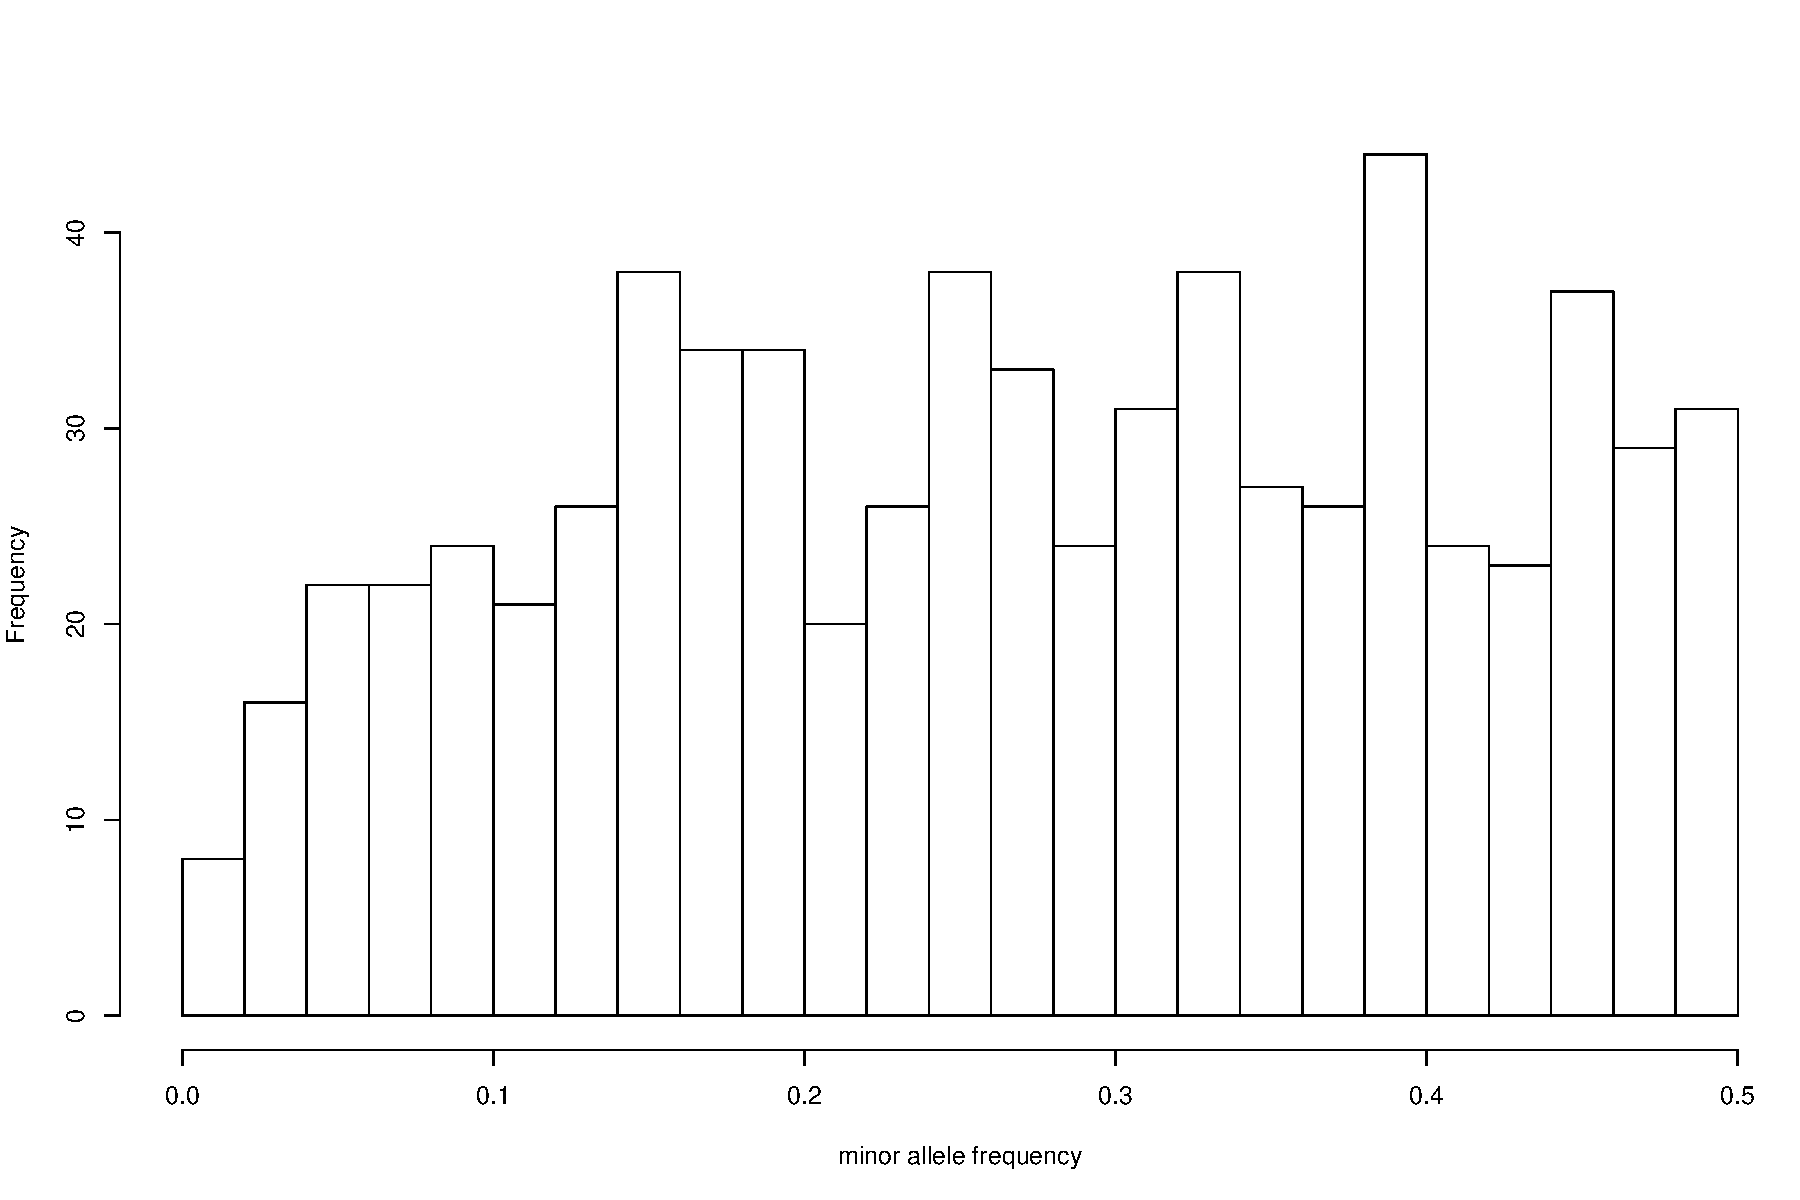
\includegraphics{figs/vignette-004}
\caption{Kernel density estimate of the minor allele frequency of the 696 SNP markers in \texttt{maize} data.}
\label{fig:histmaf}
\end{figure}

In experimental data usually missing values occur in genotypic data due to different reasons.  
The function \texttt{codeGeno} could be used to impute missing values by chance or according to family structure using the following rules:
\begin{description}
\item[with population structure]
Suppose an observation $i$ is missing (NA) for a marker $j$ in population $k$. If marker $j$ is fixed in population $k$, 
the imputed value will be the fixed allele. If marker $j$ is segregating in population $k$, 
the value is 0 with probability 0.5 and 2 with probability 0.5.
\item[without population structure] The missing values for a marker $j$ are sampled from the allele distribution of marker $j$.
\end{description}   
An alternative is to treat missing values as heteroyzgous genotypes using argument \texttt{replace.value} of function \texttt{codeGeno}.      
A complete data set of genotypes is important if marker data should be used to estimate relatedness between individuals.
To illustrate imputing of missing values, 200 entries of the marker matrix are selected, the values saved and these entries are coded as \texttt{NA}. 
\begin{Schunk}
\begin{Sinput}
> marker <- as.matrix(marker)
> ind1 <- sample(1:nrow(marker), 200)
> ind2 <- sample(1:ncol(marker), 200)
> posNA <- cbind(ind1, ind2)
> original <- marker[posNA]
> marker[posNA] <- NA
\end{Sinput}
\end{Schunk}
Note that missing values in the marker data must be coded as \texttt{NA}.                                                                                                                                                                                    
The  1250 genotypes in the \texttt{maize} data comprise 25 \textit{half sib} families with 50 genotypes in each family. The genotypes are ordered by family, thus population structure simply is
\begin{Schunk}
\begin{Sinput}
> pop <- rep(1:25, each = 50)
\end{Sinput}
\end{Schunk}
Recoding of the marker data and imputing of the missing  values using population structure is done as follows
\begin{Schunk}
\begin{Sinput}
> marker1 <- codeGeno(marker, impute = TRUE, pop)
\end{Sinput}
\begin{Soutput}
approximative run time  0  seconds 
 ... 
total number of missing values                : 200 
number of imputations by family structure     : 123 
number of random imputations                  : 77 
approximate fraction of correct imputations : 0.808 
\end{Soutput}
\end{Schunk}
A report is printed on the screen which informs about the number of imputations performed either according to family structure $n_F$ or chance $n_R$. The approximate fraction of correct imputations is $\frac{n_F + 0.5n_R}{n_F+n_R}$. For simulated data  
original values are known. The quality of the classification of the missing values is judged in the following cross-table of imputed and original values
\begin{Schunk}
\begin{Sinput}
> imputed <- marker1[posNA]
> (t1 <- table(original, imputed))
\end{Sinput}
\begin{Soutput}
        imputed
original   0   2
       0 128  18
       2  24  30
\end{Soutput}
\end{Schunk}
The fraction of correct replacements is
\begin{Schunk}
\begin{Sinput}
> sum(diag(t1))/sum(t1)
\end{Sinput}
\begin{Soutput}
[1] 0.79
\end{Soutput}
\end{Schunk}
which is much higher than the expected fraction of correct imputations without family structure which equals 0.5. At the moment there is no possibility to impute missing values using information of other (flanking) markers. This is the best alternative if no population structure is given. For this purpose, package function \texttt{fill.geno} of package \texttt{qtl} could be used. 

In an analysis of genotypic data molecular markers with a small minor allele frequency and/or many missing values are discarded using arguments \texttt{maf} and \texttt{nmiss} of function \texttt{codeGeno}. 
In this case all markers with more than
\texttt{nmiss}$\cdot 100\%$ missing values are discarded before recoding and after recoding only markers with a minor allele frequency $>$ \texttt{maf} are returned by the function. 
By default, no markers are selected by one of both criteria, thus \texttt{maf}=\texttt{nmiss}=0.
                                       
%To summarize, the steps presented in Algorithm \ref{alg:codeGeno} are performed.

%\begin{algorithm}[H]
%\SetAlgoLined
%\KwData{\texttt{data.frame} or \texttt{matrix} with $M$ biallelic marker data coded arbitrarily and missing data for $n$ genotypes $g_{ij}$.}
%\KwResult{Marker data without missing vaules with minor allele coded as 2 and major allele coded as 0.}
%\For{$j=$1 to $M$ }{
%\lIf{\% missings $>$ nmiss$\cdot 100\%$} discard marker $j$\;
%\lElse{}{
%Create frequency table for allele $A_1$ and $A_2$ for marker $j$\;
%Order alleles decreasingby their frequencies $f(A_{(1)}) > f(A_{(2)})$\;
%}
%\For{$i=1$ to $n$}{
%\lIf{$g_{ij}$ = $A_{(1)}$}{
%$g_{ij}$ = 0\;
%}
%\lIf{$g_{ij}$ = $A_{(2)}$}{
%$g_{ij}$ = 2\;
%}
%\lElse{}{
%\lIf{$\bs{g}_i$ is segregating in family of genotype $i$}{
%$g_{ij} = \left\{ \begin{array}{ll} 0 & p=0.5 \\ 2 & p=0.5 \end{array} \right. $\;
%}
%\lElse{}{
%$g_{ij}$ = fixed allele in family of genotype $i$\;
%}}
%}
%}
%Recode alleles if minor allele changed due to imputing of missing values\;
%Reject markers with minor allele frequency $<$ \texttt{maf}\;
%\caption{Umkodieren der Allele und Ersetzen von fehlenden Werten}
%\label{alg:codeGeno}
%\end{algorithm}     


\section{Linkage Disequilibrium}\label{sec:LinkageDisequilibrium}

\textit{Linkage Disequilibrium} (LD) is defined as a non-random association between polymorphisms of two or more molecular markers (usually part of same linkage group). It appears because many individuals can inherit a linked allele pair from an ancestor without any recombination event.  Average LD over the whole genome is important as it influences prospects of genomic selection. 
It is calculated as the difference between observed and expected (assuming random distributions) allelic frequencies. There are many possibilities to compute LD from genotypic data, see \citet{Foulkes2009} using \texttt{genetics} package. In \texttt{synbreed} package, LD between two loci $i$ and $j$ denoted as $LD_{ij}$
is computed as coefficient of determination $R^2$ of a regression of $\bf x_i$ on $\bf x_j$, where $\bf x_i$ and $\bf x_j$ are a $n$-dimensional vectors containing marker data of $n$ individuals. This equals squared correlation coefficient of both data vectors, thus
$$  LD_{ij} = r(\bf x_i,\bf x_j)^2 .$$
Relationship between markers is assumed to decrease as their distance on chromosome increases. To visualize this decline, the LD is plotted against the distance on the chromosome. 
For \texttt{maize} we plot the LD for the marker located on the first (out of 10) chromosomes using function \texttt{LDDist}. This function provides several possibilities for graphical visualisation. To visualize LD decay on first chromosome of \texttt{maize} data, use
\begin{Schunk}
\begin{Sinput}
> data(maize)
> marker <- codeGeno(maize.geno[, -1])
> LDDist(marker, maize.marker.pos$chr, maize.marker.pos$pos, 
+     chr = 1)
\end{Sinput}
\end{Schunk}
Figure \ref{fig:subfig1} and  \ref{fig:subfig2} present two possibilites for graphical visulisation using different values for argument \texttt{type}.

\begin{figure}[!ht]
\centering
\subfigure[Scatterplot using \texttt{type="p"}]{
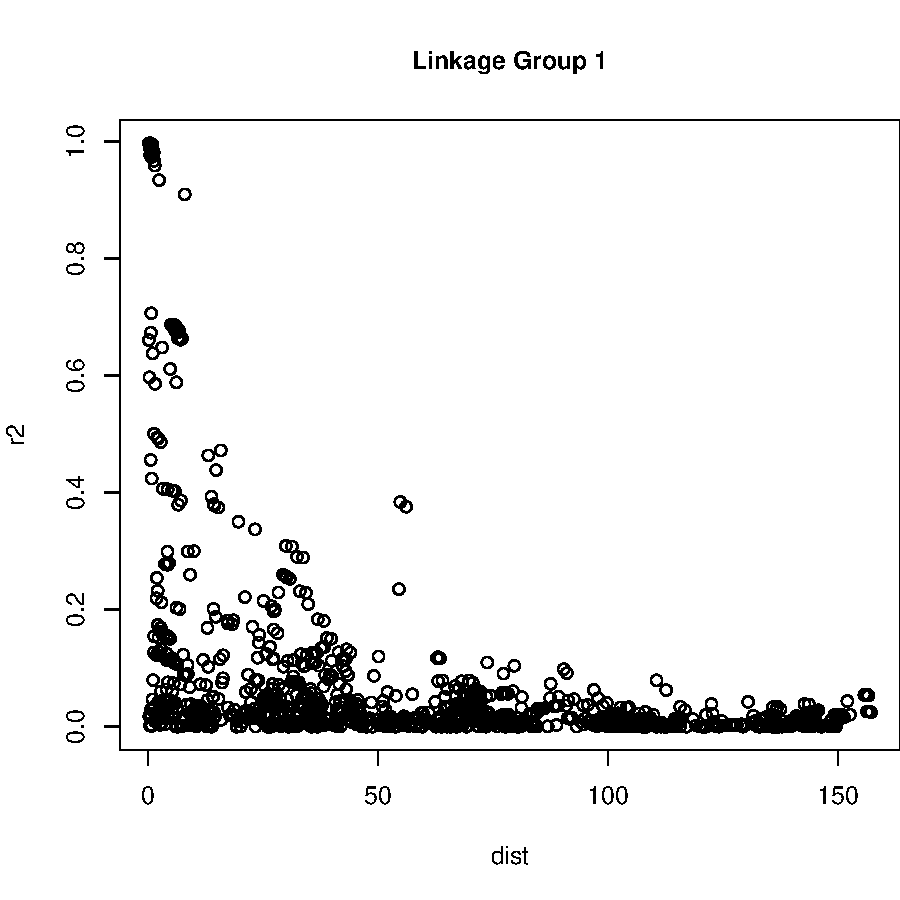
\includegraphics{figs/vignette-011}
\label{fig:subfig1}
}\qquad
\subfigure[Stacked histogram using \texttt{type="bars"}]{
\includegraphics{figs/vignette-012}
\label{fig:subfig2}
}
\caption{LD  vs distance for first chromosome of \texttt{maize} data. }
\end{figure}

As genotypes are effected by selection due in simulation progress for many generations, LD above 0.6 is only observable up to a distance of 10 cM for the first chromosome, see Figure \ref{fig:subfig2} . Another type of graphic is a heatmap of LD for markers located on the same chromosome. LD heatmap for pairwise LD of markers on the first chromosome is obtained by function \texttt{LDMap} which is simply a wrapper for funtion \texttt{LDheatmap} of package \texttt{LDheatmap}.


\begin{figure}[!ht]
\begin{Schunk}
\begin{Sinput}
> LDMap(marker[, chr1], maize.marker.pos$chr[chr1], maize.marker.pos$pos[chr1])
\end{Sinput}
\end{Schunk}
\includegraphics{figs/vignette-013}
\caption{LD heatmap for markers on first chromosome of \texttt{maize} data.}
\label{fig:LDMap}
\end{figure} 

Strong LD could be observed between the markers on the ''left'' margin of Chromosome 1, compare Figure \ref{fig:LDMap}.



\section{Pedigree}\label{sec:Pedigree}     
                               
An important source of information in breeding programs is pedigree information. Especially in animal breeding, pedigree is recorded over many generations. The pedigree usually consists 
of a list of individuals (animals or plants) of the current generation which is the subject of analysis and their ancestors (for which often no phenotypic data is available). The pedigree is sorted by generation, beginning with the individuals with unknown parents. An example for a pedigree with five individuals belonging to 4 generations is given below. Parents of A and B are unknown.

\begin{table}[!ht]
\centering
\begin{tabular}{cccc}
\hline
ID & Par1 & Par2 & gener \\
\hline
A & - & - & 0 \\
B & - & - & 0 \\
C & A & B & 1 \\
D & A & C & 2 \\
E & D & B & 3 \\
\hline
\end{tabular}
\end{table}

 In \texttt{synbreed} class "pedigree" should be used for handling pedigree information. An object of class "pedigree" consists of a \texttt{data.frame} with at least variables \texttt{ID}, \texttt{Par1}, \texttt{Par2} and \texttt{gener}.
The function \texttt{create.pedigree} creates an object of class  "pedigree" for a given set of individuals and the pair of parents. Note that unknown parents are coded as "0" in \texttt{synbreed} package and generation starts with 0. The generation can be specified by the user or optional computed by the function.

Suppose we have the pedigree structure of the example. This structure is carried into \texttt{synbreed} package with the following commands
\begin{Schunk}
\begin{Sinput}
> id <- c("A", "B", "C", "D", "E")
> par1 <- c(0, 0, "A", "A", "D")
> par2 <- c(0, 0, "B", "C", "B")
> ped <- create.pedigree(id, par1, par2)
> ped
\end{Sinput}
\begin{Soutput}
  ID Par1 Par2 gener
1  A    0    0     0
2  B    0    0     0
3  C    A    B     1
4  D    A    C     2
5  E    D    B     3
\end{Soutput}
\end{Schunk}
An object of class "pedigree" could be visualized with generic plotting function for S3 class "pedigree".
 
\begin{figure}[!ht] 
\begin{Schunk}
\begin{Sinput}
> plot(ped)
\end{Sinput}
\end{Schunk}
\includegraphics{figs/vignette-015}
\end{figure}    
      
It is possible to simulate a pedigree structure with function \texttt{simul.pedigree}. As arguments,
the number of generations to simulate and the number of individuals in each generation has to be specified. By default, random mating 
is assumed in each generation. As there are no further restrictions, it is possible that inbreeds could be generated when parent 1 equals parent 2.
To simulate a pedigree with 6 generations and 4, 6, 7, 9, 10 and 10 individuals in each generation, use
\begin{Schunk}
\begin{Sinput}
> set.seed(123)
> ped.simul <- simul.pedigree(gener = 6, ids = c(4, 6, 
+     7, 9, 10, 10))
\end{Sinput}
\end{Schunk}
The resulting pedigree is visualized in Figure \ref{fig:simupedi}. A basic summary of the pedigree is given by the generic \texttt{summary} method for class ''pedigree''.
\begin{Schunk}
\begin{Sinput}
> summary(ped.simul)
\end{Sinput}
\begin{Soutput}
# individuals    : 46 
# Par1 (sire)    : 27 
# Par2 (dam)     : 25 
# generations    : 6 
# unknow parents : 8 
# inbred         : 5 
\end{Soutput}
\end{Schunk}

\begin{figure}[!ht]
\begin{Schunk}
\begin{Sinput}
> plot(ped.simul)
\end{Sinput}
\end{Schunk}
\includegraphics{figs/vignette-018}
\caption{Simulated pedigree structure}
\label{fig:simupedi}
\end{figure}

\section{Genotypic Means and Variances}\label{sec:theory}

This section summarazies some theory of quantitative genetics which is necessarry for the following sections. Those readers who are familiar with the concepts of genetics as presented in \citet{Falconer1996} or \citet{Bernardo2002}
may skip this section. All formulas are presented for the one-locus model in a breeding population.

We consider a single locus with two alleles $A_1$ and $A_2$ so that genotypes $A_1A_1$, $A_1A_2$ and $A_2A_2$ are possible. The phenotypic mean $G_{ij}$ of individuals having the $A_iA_j$ genotype can be expressed as
$$ P_{ij} = G_{ij} + e_{ij}$$
where  $G_{ij}$ is the genotypic value of $A_iA_j$ and $e_{ij}$ is the nongenetic residual which is assumed to be unrelated to genotypic value. The genotypic value can be further divided into
$$ G_{ij} = \mu + \alpha_i + \alpha_j + \delta_{ij}$$
where $\mu$ is the population mean, $\alpha_i$ is the effect of the $A_i$ allele which is defined as the average effect of an allele. This is the difference of the mean of those individuals who received $A_i$ allele
from one parent and the other allele at random from the population. The effect $\alpha_j$ is defined in a similar way. The breeding value of the $A_iA_j$ genotype is defined as the sum of $\alpha_i$ and $\alpha_j$. The term $\delta_{ij}$ is the    dominance deviation of the $A_iA_j$ genotype. Dominance deviation is due to the interaction of both alleles at one locus.   

On a population level, we consider the variance of the effects mentioned above. Phenotypic variance $V_P$ can be partioned into genotypic variance $V_G$ and non genetic variance $V_E$. The genetic variance within one locus is divided into addtive variance and dominance variance, thus $V_G=V_A+V_D$. If more than one locus
is considered, additional epistatic variance $V_I$ occurs which is due to interactions between different loci. Epistatic variance consists in two locus model of additive-additive variance $V_{AA}$, additive-dominace variance $V_{AD}$ and dominance-dominance variance $V_{DD}$ due to the two-way interactions of additive and dominance effects.

An important concept in breeding is the covariance between relatives which is a function of the probability that two alleles are identical by descent and genetic variance components. Suppose we have the pedigree structure as shown in Figure \ref{fig:pedigree}.

\setlength{\unitlength}{1cm}
\begin{figure}[!ht]
\centering
\begin{picture}(4.5,4.5)
\put(1,4){A}
\put(2,4){B}
\put(3,4){C}
\put(4,4){D}
\put(1,3.8){\vector(1,-4){0.51}}
\put(2.1,3.8){\vector(-1,-4){0.51}}
\put(3,3.8){\vector(1,-4){0.51}}
\put(4.1,3.8){\vector(-1,-4){0.51}}
\put(1.5,1){X}
\put(3.5,1){Y}
\put(1.3,0.5){$A_iA_j$}
\put(3.3,0.5){$A_kA_l$}
\end{picture}
\caption{Pedigree of X and Y.}
\label{fig:pedigree}
\end{figure}

Covariance between relatives is due to alleles that are identical by descent (IBD), denoted by the $\equiv$ symbol. There are four possibilities that two alleles in X and Y are IBD and covariance due to breeding values is given by
\begin{eqnarray*}
\Cov_{\alpha} &=& P(A_i \equiv A_k)\Cov(\alpha_i,\alpha_k)+ P(A_i \equiv A_l)\Cov(\alpha_i,\alpha_l)\\
&+& P(A_j \equiv A_k)\Cov(\alpha_j,\alpha_k) + P(A_j \equiv A_l)\Cov(\alpha_j,\alpha_l) \\
&=& 2f_{XY}V_A
\end{eqnarray*}
where $f_{XY}$ is the coefficient of coancestry \citep{Wright1922} which is defined as
\begin{eqnarray}
f_{XY} &=& P(X \equiv Y) \nonumber \\
&=& \frac{1}{4}\left[ P(x_1 \equiv y_1) + P(x_1 \equiv y_2) + P(x_2 \equiv y_1) + P(x_2 \equiv y_2)\right].
\end{eqnarray}
Covariance between relatives according to dominance and epistatic variances can be derived in a similar way, see \citet{Bernardo2002} and next section. 
 



  

\section{Estimation of Relatedness}\label{sec:RelationshipMatrices}  

This section presents methods to estimate relatedness between a set of individuals. The goal is to set up a variance-covariance matrix for the individuals. Relatedness between individuals refers to their covariance due to some kind of genetic effect.
In classical breeding programs, pedigree information is used to compute \textit{expected} relatedness. Thus the entries of the variance-covariance matrix are derived by the formulas of the previous section.   If molecular markers are available, \textit{observed} relatedness between individuals could be estimated using similarity measures for genotypic data.

\subsection{Based on Pedigree}

The computation of the pedigree based relatedness in \texttt{synbreed} starts with the gametic relationship. A gamete is the genetic unit that an individual passes to its offspring. The genotype of a diploid individual at one locus consists of two alleles. 
Suppose there is an individual C with parents A and B. Individual C has to alleles $C_1$ and $C_2$. The source of allele $C_1$ is Parent A, thus allele $C_1$ could either be IBD to $A_1$ or $A_2$ which are the alleles (and possible gametes) of A. Allele $C_2$ was inherited of parent B, thus it could be IBD to $B_1$ or $B_2$ which are the alleles of B. 
To compute the gametic relationship start with an expanded table with two alleles for each individual. 
 
\begin{table}[!ht]
\centering
\begin{tabular}{cccc}
\hline
ID & Allele & Par1 & Par2 \\
\hline
A & $A_1$ & - & - \\
A & $A_2$ & - & - \\
B & $B_1$ & - & - \\
B & $B_2$ & - & - \\
C & $C_1$ & $A_1$ & $A_2$ \\
C & $C_2$ & $B_1$ & $B_2$ \\
D & $D_1$ & $A_1$ & $A_2$ \\
D & $D_2$ & $C_1$ & $C_2$ \\
E & $E_1$ & $D_1$ & $D_2$ \\
E & $E_2$ & $B_1$ & $B_2$ \\
\hline
\end{tabular}
\end{table}

This table is converted into the gametic relationship $\bf G$ matrix which is of order $2n$, if the number of individuals is $n$. The entires of $\bf G$ are the probability that two alleles $A_1$ and $A_2$ are identical by
descent (IBD), denoted as $P(A_1 \equiv A_2)$. Thus diagonal values are always 1. If parents are unknown, they are assumed as progeny of a random mating population. In this case the off-diagonals are zero. The gametic relationsship matrix is constructed recursively, starting with the first 
generation in pedigree. 
The combination of $2^2=4$ alleles that describe the relationship of progeny A with parent C are computed as follows
\begin{eqnarray*} 
P(A_1 \equiv C_1) &=& 0.5 \cdot \left[P(A_1 \equiv A_1) + P(A_1 \equiv A_2)\right]  \\
P(A_1 \equiv C_2) &=& 0.5 \cdot \left[P(A_1 \equiv B_1) + P(A_1 \equiv B_2)\right]  \\
P(A_2 \equiv C_1) &=& 0.5 \cdot \left[P(A_2 \equiv A_1) + P(A_2 \equiv A_2)\right]  \\
P(A_2 \equiv C_2) &=& 0.5 \cdot \left[P(A_2 \equiv B_1) + P(A_2 \equiv B_2)\right]   
\end{eqnarray*}
The only nonzero probability in the equations above is $P(A_1 \equiv A_1)$ which is 1. The gametic relationship for all individuals of a given pedigree is obtained as follows
\begin{Schunk}
\begin{Sinput}
> G <- kinship(ped, ret = "gam")
> G
\end{Sinput}
\begin{Soutput}
      A_1   A_2   B_1   B_2 C_1  C_2   D_1   D_2   E_1   E_2
A_1 1.000 0.000 0.000 0.000 0.5 0.00 0.500 0.250 0.375 0.000
A_2 0.000 1.000 0.000 0.000 0.5 0.00 0.500 0.250 0.375 0.000
B_1 0.000 0.000 1.000 0.000 0.0 0.50 0.000 0.250 0.125 0.500
B_2 0.000 0.000 0.000 1.000 0.0 0.50 0.000 0.250 0.125 0.500
C_1 0.500 0.500 0.000 0.000 1.0 0.00 0.500 0.500 0.500 0.000
C_2 0.000 0.000 0.500 0.500 0.0 1.00 0.000 0.500 0.250 0.500
D_1 0.500 0.500 0.000 0.000 0.5 0.00 1.000 0.250 0.625 0.000
D_2 0.250 0.250 0.250 0.250 0.5 0.50 0.250 1.000 0.625 0.250
E_1 0.375 0.375 0.125 0.125 0.5 0.25 0.625 0.625 1.000 0.125
E_2 0.000 0.000 0.500 0.500 0.0 0.50 0.000 0.250 0.125 1.000
attr(,"class")
[1] "relationshipMatrix"
\end{Soutput}
\end{Schunk}
The resulting object \texttt{G} is of class "relationshipMatrix" which is the general class for all variance-covariance matrices due to genetic effects (additive, dominance or epistatic). To derive the variance-covariance matrix due to an genetic effect,
one has to multiply this matrix with the corresponding variance component ($V_A$, $V_D$ or $V_I$) as shown below. Once the gametic relationship is computed, it could be converted in the additive numerator relationship matrix $\bf A$ which is due to additive genetic effects (breeding values) or the dominance relationship matrix $\bf D$ which is due to dominance effects.  

In case of inbreeding, the entry in \texttt{G} of allele $A_1$ and allele $A_2$ of an individual X equals his inbreeding coefficient $$F_X=P(A_1 \equiv A_2).$$ For example, the inbreeding coefficent of individual D is
\begin{Schunk}
\begin{Sinput}
> as.numeric(G["D_1", "D_2"])
\end{Sinput}
\begin{Soutput}
[1] 0.25
\end{Soutput}
\end{Schunk}
which is nonzero because individuals A and C, which are the parents of D, are relatives. 

 The additive relationship between individuals X and Y is given by
$$ A_{XY} = \begin{cases} 1+F_X, & X=Y \\ 2f_{XY}, & X\neq Y \end{cases}$$
where $f_{XY}$ is the coefficient of coancastry between X and Y. The additive numerator relationship is of order $n$ and derived for a given pedigree as
\begin{Schunk}
\begin{Sinput}
> A <- kinship(ped, ret = "add")
> A
\end{Sinput}
\begin{Soutput}
      A     B     C    D     E
A 1.000 0.000 0.500 0.75 0.375
B 0.000 1.000 0.500 0.25 0.625
C 0.500 0.500 1.000 0.75 0.625
D 0.750 0.250 0.750 1.25 0.750
E 0.375 0.625 0.625 0.75 1.125
attr(,"class")
[1] "relationshipMatrix"
\end{Soutput}
\end{Schunk}
The relationship between individuals A and C is 0.5 which is the expected value for parent-offspring relation \citep{Bernardo2002}. Note that the diagonals of $\bf A$ are $1+F_i$ for $i=1,...,n$. 
Inbreeding coefficients could easily be obtained as
\begin{Schunk}
\begin{Sinput}
> diag(A) - 1
\end{Sinput}
\begin{Soutput}
    A     B     C     D     E 
0.000 0.000 0.000 0.250 0.125 
\end{Soutput}
\end{Schunk}
Sometimes the kinship matrix is required, which is half of the additive numerator relationship matrix. It is obtained by
\begin{Schunk}
\begin{Sinput}
> K <- kinship(ped, ret = "kin")
\end{Sinput}
\end{Schunk}

%Additionally it is possible to derive the dominance relationship matrix $\bf D$ out of $\bf G$. The dominance between individuals $X$ and $Y$ is given by
%$$ D_{XY} = \begin{cases} 1-F_X, & X=Y \\ t_{XY}, & X\neq Y \end{cases}$$
%where $t_{XY}$ being the coefficient of dominance covariance defined as
%\begin{eqnarray*}
%t_{XY} &=& P(X_1 \equiv Y_1 \neq X_2 \equiv Y_2) +  P(X_1 \equiv Y_2 \neq X_2 \equiv Y_1) \\
%&=&  P(Y_1 \neq X_2)P(Y_1 \neq Y_2)\left[ P(X_1 \equiv Y_1)P(X_2 \equiv Y_2)+P(X_2 \equiv Y_1)P(X_1 \equiv Y_2) \right] \\
%&=& (1-F_X)(1-F_Y)\left[ P(X_1 \equiv Y_1)P(X_2 \equiv Y_2)+P(X_2 \equiv Y_1)P(X_1 \equiv Y_2) \right].
%\end{eqnarray*}
%Note that for a completely homozygous line $X$ dominance is zero because $F_X=1$. Dominance relationship matrix 
%for the example pedigree is obtained  by
%<<>>=
%D <- kinship(ped,ret="dom")
%D
%@
Dominance covariance matrix is computed if argument \texttt{ret="dom"} is used. Variance-covariance matrices for epistatic effects as additive-additive (AA), additive-dominance (AD) or dominance-dominance (DD) are the products of the corresponding variance-covariance matrices for additice and dominace effects.                               
Models for genomic selection can be extended by these effects, but the contribution of three-way or higher interactions is usually small \citep{Bernardo2002}.  


\subsection{Based on marker data}

                 
Relatedness based on marker is an alternative to estimate relationship instead of using additive numerator relationship matrix based on pedigree. Marker data could be used to estimate relationship between relatives
more precise than the numerator relationship based on pedigree as it takes into account the Mendelian sampling effect. Two methods for the construction of a relationship matrix based on marker data are implemented in the \texttt{synbreed} package: genomic relationship according to vanRaden \citep{vanRaden2008} and according to Roger's distance  \citep{Rogers1972}.  Both methods are kinds of similarity measures which compare
the number of alleles that two individuals share.

For vanRaden, the SNP genotypes are coded as the number of copies of the minor allele, i.e., 0, 1 or 2 (no missing values allowed). Thus the marker data could be the result of a call of \texttt{codeGeno} when imputing for the missing values was performed or the missing values were replaced with the value 1.
The genomic relationship matrix according to vanRaden for $n$ individuals and $p$ molecular markers is computed as
\begin{equation}\label{eq:vanRaden}
\frac{\bf{Z}\bf{Z}'}{2\sum_{i=1}^p p_i(1-p_i)},
\end{equation}
where $\bf{Z}=\bf{M}-\bf{P}$ and $\bf{M}$ is the $n \times p$ marker matrix and $\bf{P}$ contains the allele frequencies multiplied by 2. In \eqref{eq:vanRaden} $p_i$ is the allele frequency of marker $i$.  As an example we look at the marker data of 6 individuals genotyped with 8 SNP markers. Let
$$ \bf M = \begin{pmatrix}  2 & 0 & 0 & 2 & 2 & 0 & 0 & 0 \\ 
   2 & 0 & 2 & 2 & 2 & 0 & 2 & 2 \\ 
   2 & 0 & 2 & 2 & 0 & 0 & 2 & 0 \\ 
   0 & 0 & 2 & 2 & 0 & 0 & 2 & 0 \\ 
   0 & 0 & 2 & 0 & 0 & 0 & 2 & 0 \\ 
   2 & 2 & 2 & 2 & 0 & 0 & 0 & 2 \\  
   \end{pmatrix}, $$
then it holds that
$$ \bf P = \begin{pmatrix}  1.33 & 0.33 & 1.67 & 1.67  & 0.67 & 0 &  1.33&  0.67 \\ 
   1.33 & 0.33 & 1.67 & 1.67  & 0.67 & 0 &  1.33&  0.67 \\ 
   1.33 & 0.33 & 1.67 & 1.67  & 0.67 & 0 &  1.33&  0.67 \\  
   1.33 & 0.33 & 1.67 & 1.67  & 0.67 & 0 &  1.33&  0.67 \\ 
   1.33 & 0.33 & 1.67 & 1.67  & 0.67 & 0 &  1.33&  0.67 \\  
   1.33 & 0.33 & 1.67 & 1.67  & 0.67 & 0 &  1.33&  0.67 \\   
   \end{pmatrix} $$
 $$    \bf Z = \begin{pmatrix}   0.67 & -0.33 & -1.67 & 0.33 & 1.33 & 0.00 & -1.33 & -0.67 \\ 
  0.67 & -0.33 & 0.33 & 0.33 & 1.33 & 0.00 & 0.67 & 1.33 \\ 
   0.67 & -0.33 & 0.33 & 0.33 & -0.67 & 0.00 & 0.67 & -0.67 \\ 
  -1.33 & -0.33 & 0.33 & 0.33 & -0.67 & 0.00 & 0.67 & -0.67 \\ 
   -1.33 & -0.33 & 0.33 & -1.67 & -0.67 & 0.00 & 0.67 & -0.67 \\ 
   0.67 & 1.67 & 0.33 & 0.33 & -0.67 & 0.00 & -1.33 & 1.33 \\ 
   \end{pmatrix}
  $$  
  and 
  $$ \bf Z \bf Z ' = \begin{pmatrix}  
   7.44 & 0.11 & -1.22 & -2.56 & -3.22 & -0.56 \\ 
   0.11 & 4.78 & -0.56 & -1.89 & -2.56 & 0.11 \\ 
   -1.22 & -0.56 & 2.11 & 0.78 & 0.11 & -1.22 \\ 
   -2.56 & -1.89 & 0.78 & 3.44 & 2.78 & -2.56 \\ 
   -3.22 & -2.56 & 0.11 & 2.78 & 6.11 & -3.22 \\ 
   -0.56 & 0.11 & -1.22 & -2.56 & -3.22 & 7.44 \\
     \end{pmatrix}
  $$                                                                                   
with the denominator being $2\sum_{i=1}^p p_i(1-p_i)=2.611$. Correcting with the allele frequencies gives more weight to individuals that share a rare allele. To compute the genomic relationship according to vanRaden, matrix $\bf M$ is passed to the function \texttt{vanRaden}  
\begin{Schunk}
\begin{Sinput}
> M <- matrix(data = c(2, 0, 0, 2, 2, 0, 0, 0, 2, 0, 2, 
+     2, 2, 0, 2, 2, 2, 0, 2, 2, 0, 0, 2, 0, 0, 0, 2, 2, 
+     0, 0, 2, 0, 0, 0, 2, 0, 0, 0, 2, 0, 2, 2, 2, 2, 0, 
+     0, 0, 2), nrow = 6, byrow = TRUE)
> vR <- vanRaden(M)
> round(vR, 3)
\end{Sinput}
\begin{Soutput}
       [,1]   [,2]   [,3]   [,4]   [,5]   [,6]
[1,]  2.851  0.043 -0.468 -0.979 -1.234 -0.213
[2,]  0.043  1.830 -0.213 -0.723 -0.979  0.043
[3,] -0.468 -0.213  0.809  0.298  0.043 -0.468
[4,] -0.979 -0.723  0.298  1.319  1.064 -0.979
[5,] -1.234 -0.979  0.043  1.064  2.340 -1.234
[6,] -0.213  0.043 -0.468 -0.979 -1.234  2.851
attr(,"class")
[1] "relationshipMatrix"
\end{Soutput}
\end{Schunk}
Note the object \texttt{vR} is again of class "relationshipMatrix". Negative values indicate pairs of individuals sharing fewer alleles than expected by the allele frequencies.   

Another possibility is to compute the genomic relationship matrix according to Roger's distance. Roger's distance is computed as 
\begin{equation}
d=\frac{1}{p}\sum_{i=1}^p \sqrt{1/2 \sum_{j=1}^{n_i}(p_{ij}-q_{ij})^2}
\end{equation}
where $p$ is the number of markers and $n_i$ is the number of alleles for marker $i$. Let $p_{ij}$ and $q_{ij}$ denote the allele frequencies of allele $j$ for marker $i$ respectively. Note that marker data should be coded $-1$ and $1$ for homozygous genotypes and 0 for heterozygous. If marker data is coded as 0/1/2, data is transformed by function \texttt{rogers}, which computes relationship based on Roger's distance. Using transformation of \citet{Hayes2008} rogers distance is related to relationship as
$$ f=\frac{s-s_{min}}{1-s_{min}}, $$
with similarity measure $s=1-d$ and $s_{min}$ minimum of all $\frac{n}{2}(n+1)$ values for $s$. Using rogers distance to compute relationship based on marker data gives
\begin{Schunk}
\begin{Sinput}
> ro <- rogers(M, correction = "Hayes")
> round(ro, 3)
\end{Sinput}
\begin{Soutput}
     [,1] [,2] [,3] [,4] [,5] [,6]
[1,]  2.0  0.8  0.8  0.4  0.0  0.4
[2,]  0.8  2.0  1.2  0.8  0.4  0.8
[3,]  0.8  1.2  2.0  1.6  1.2  0.8
[4,]  0.4  0.8  1.6  2.0  1.6  0.4
[5,]  0.0  0.4  1.2  1.6  2.0  0.0
[6,]  0.4  0.8  0.8  0.4  0.0  2.0
attr(,"class")
[1] "relationshipMatrix"
\end{Soutput}
\end{Schunk}
Note that function \texttt{rogers} returns $2f$ which is the relationship between individuals.


\subsection{Doubled haploid lines}

In modern plant breeding programs in maize, doubled haploid (DH) lines are used as parents in crosses. DH lines are fully inbred and thus have an inbreeding coefficient of 1. This has to be taken into account, when the relationship matrix in a pedigree with DH lines is computed.  As an example the \texttt{maize} data is taken.
\begin{Schunk}
\begin{Sinput}
> data(maize)
> head(maize.ped)
\end{Sinput}
\begin{Soutput}
  ID Par1 Par2 DH
1  1    0    0  1
2  2    0    0  1
3  3    0    0  1
4  4    0    0  1
5  5    0    0  1
6  6    0    0  1
\end{Soutput}
\end{Schunk}
Last column is a logical that indicates DH lines.First, the additive numerator relationship matrix is computed. There are 1276 DH lines and 25 non DH lines in the pedigree. For DH lines special treatment is necessary, as the inbreeding coefficient must be 1 and no heterozygous genotypes occur.. An argument \texttt{DH} is available for function \texttt{kinship} where
for each individual in the pedigree it specified whether this is a DH line or not. This information is available for the \texttt{maize} data. To obtain the additive numerator relationship matrix, use 
\begin{Schunk}
\begin{Sinput}
> ped.maize <- create.pedigree(maize.ped$ID, maize.ped$Par1, 
+     maize.ped$Par2)
> A.maize <- kinship(ped.maize, DH = maize.ped$DH, ret = "add")
> dim(A.maize)
\end{Sinput}
\begin{Soutput}
[1] 1301 1301
\end{Soutput}
\end{Schunk}
All inbreeding coefficients of DH lines are now one
\begin{Schunk}
\begin{Sinput}
> head(diag(A.maize) - 1)
\end{Sinput}
\begin{Soutput}
1 2 3 4 5 6 
1 1 1 1 1 1 
\end{Soutput}
\end{Schunk}

\subsection{Visualization of relationship matrices}

In most cases a relationship matrix is too big to print on screen. There are two possibilities for visualization of an object of class "relationshipMatrix" in \texttt{synbreed} package. A generic \texttt{summary} method is defined which gives the important characteristics of a relationship matrix. Use
\begin{Schunk}
\begin{Sinput}
> summary(A.maize)
\end{Sinput}
\begin{Soutput}
Dimension         : 1301 x 1301 
Rank              : 1276 
Range             : 0 -- 2 
# of unique values: 6 
\end{Soutput}
\end{Schunk}
to get the summary for the pedigree based additive relationship matrix of the \texttt{maize} data. Another possibility is the \texttt{plot} method which could be applied
to an object of class "relationshipMatrix". This gives a heatmap of the entries of the relationship matrix
%\begin{figure}
%<<fig=TRUE>>=
%plot(A.maize[1:100,1:100])
%@
%\caption{Heatmap of pedigree based additive relationship matrix for \texttt{maize} data.}
%\label{fig:heatpedi}
%\end{figure}
%In Figure \ref{fig:heatpedi} one can see the family  structure in the data which is consiting of 25 families.

Note that objects of class "relationshipMatrix" can be written to input files appropriate for Mixed Model software as \texttt{WOMBAT} \citep{Meyer2006} or \texttt{ASReml} \citep{Gilmour2000} using function 
\texttt{write.relationshipMatrix}. File formats are \texttt{*.gin} for \texttt{WOMBAT} and \texttt{*.grm} or \texttt{*.giv} for \texttt{ASReml}.

\section{Mixed Models}\label{sec:Models}

The ultimate aim in the analysis of a breeding program is to estimate genetic effects and variance components. The basic statistical model for this purpose is a linear mixed model
\begin{equation}\label{eq:mm}
\bf y = \bf X \bf b + \bf Z \bf u + \bf e,
\end{equation}
where $\bf y$ is the $n \times 1$ vector of phenotypic records, $\bf b$ a $t \times 1$ vector of fixed effects and $\bf u$ a  $m \times 1$ vector of random effects. $\bf X$ and $\bf Z$ are the corresponding design matrices with dimension $n \times t$  and $n \times m$ respectively. The random genetic effect has distribution
$$ \bf u \sim \text{N}( \bf 0, \bf G \sigma^2_g)$$
where $\bf G$ is a genetic variance-covariance matrix. In \eqref{eq:mm} $\bf e$ denotes the $n \times 1$ vector of residuals with $ \bf e \sim \text{N}( \bf 0, \bf I_n \sigma^2)$ and $\bf I_n$ is the $n$-dimensional identity matrix.
                                                                                                                                                    
If $\bf G$ equals the additive numerator relationship matrix $\bf A$, model \eqref{eq:mm} is called \textit{animal model}. Here the random effect is usually denoted as $\bf a$ and $ \bf a \sim \text{N}( \bf 0, \bf A \sigma^2_a)$.  This model is used to estimate additive genetic effects (breeding values) based on phenotypic records and pedigree information.
 As an example we will simulate plant breeding data. A pedigree with 5 generations and 20 individuals in each generation is simulated. Phenotypic data was measured in a field trial consisting of 5 locations with two replications (blocks) within locations for each of the $n=100$ genotypes.

The simulation of phenotypes is done with the function \texttt{simul.phenotype} which simulates records based on model \eqref{eq:mm} with an overall mean as fixed effect and random effects for genotype, location and block. Random effects for location, block nested in location and residuals are i.i.d. normal with mean zero and given variance component.
Random effects for genotype are taken from a multivariate normal distribution $\text{N}( \bf 0, \bf A \sigma^2_a)$, where $\bf A$ is the numerator relationship matrix obtained by pedigree information. The additive genetic variance $\sigma^2_a$ and variance components for location, block and residual are specified by the user. 
Variance components are specified in a separate list and values used for simulation are $\sigma^2_a=10$, $\sigma^2=15$ and $0$ for location and block nested in location. Simulated data is obtained as follows
\begin{Schunk}
\begin{Sinput}
> ped <- simul.pedigree(5, 20)
> vc <- list(sigma2e = 15, sigma2a = 10, sigma2l = 0, sigma2b = 0)
> dat <- simul.phenotype(ped, Nloc = 5, Nrepl = 2, vc = vc)
> str(dat)
\end{Sinput}
\begin{Soutput}
'data.frame':	1000 obs. of  5 variables:
 $ ID   : Factor w/ 100 levels "1","10","100",..: 1 1 1 1 1 1 1 1 1 1 ...
 $ Loc  : Factor w/ 5 levels "1","2","3","4",..: 1 1 2 2 3 3 4 4 5 5 ...
 $ Block: Factor w/ 2 levels "1","2": 1 2 1 2 1 2 1 2 1 2 ...
 $ Trait: num  102.7 101.2 97 98.7 95.7 ...
 $ TBV  : num  -1.55 -1.55 -1.55 -1.55 -1.55 ...
\end{Soutput}
\end{Schunk}
Variance components for location and block are set to zero as only additive genetic effects should be considered in this example. The simulated random effects for 
genotype are called true breeding values (TBV) and returned by function \texttt{simul.phenotype}. Note that TBV for each \texttt{ID} is the same for all replications across locations and blocks.
                                                                                                                                   
Estimation of variance components with REML and prediction of random effects in model \eqref{eq:mm} could be done with function \texttt{regress} in package \texttt{regress} \citep{Clifford2006}. 
This package allows arbitrary variance-covariance matrices of random effects. Solutions for animal model with overall mean as fixed effect are obtained as 
\begin{Schunk}
\begin{Sinput}
> library(regress)
> A <- kinship(ped, ret = "add")
> A <- A %x% matrix(1, 10, 10)
> mod <- regress(Trait ~ 1, Vformula = ~A, data = dat)
> summary(mod)
\end{Sinput}
\begin{Soutput}
Maximised Residual Log Likelihood is -1950.051 

Linear Coefficients:
             Estimate Std. Error
 (Intercept)   99.897      0.762

Variance Coefficients:
             Estimate Std. Error
          A    10.349      1.938
          In   15.544      0.731
\end{Soutput}
\end{Schunk}
Note that variance-covariance matrix must be of same dimension as $y$. This could easily be obtained by using the Kronecker product to enlarge relationship matrix as data is sorted by individuals. This is shown in the code above. Estimated variance components could be used to estimate narrow-sense heritability as in \citet{Piepho2007} as
$$ \hat h^2 = \frac{\hat \sigma_a^2}{\hat \sigma_a^2 + \hat \sigma^2} = \frac{10.35}{10.35 + 15.54} = 0.4.$$
The fitted model contains only one random effect, thus estimated breeding values are obtained as
\begin{Schunk}
\begin{Sinput}
> ebv <- mod$predicted - mod$fitted
\end{Sinput}
\end{Schunk}
as \texttt{predicted} equals $\bf \hat y$ and \texttt{fitted} contains estimated overall mean $\bf \hat mu$ and $\bf \hat a =\bf \hat y - \bf \hat mu$. Correlation between observed and estimated phenotypes (also called \textit{predictive ability} of the model, see \citet{Legarra2008}) is
\begin{Schunk}
\begin{Sinput}
> y <- dat$Trait
> cor(ebv, y)
\end{Sinput}
\begin{Soutput}
          [,1]
[1,] 0.5823288
\end{Soutput}
\end{Schunk}
As true breeding values are known in simulate, also correlation between estimated and true genetic effect (called \textit{accuracy} of the model) is available as
\begin{Schunk}
\begin{Sinput}
> tbv <- dat$TBV
> cor(ebv, tbv)
\end{Sinput}
\begin{Soutput}
          [,1]
[1,] 0.9067806
\end{Soutput}
\end{Schunk}

\section{Genomic Selection} \label{sec:genomicSelection}

In this section, all steps that are necessary to derive (genomic) breeding values out of genotypic and phenotypic data are presented using \texttt{maize} data. Different models that make use of pedigree and/or marker data
are compared due to estimated effects and variance components.

First, additive relationship matrix based on pedigree is created
\begin{Schunk}
\begin{Sinput}
> data(maize)
> ped.maize <- create.pedigree(maize.ped$ID, maize.ped$Par1, 
+     maize.ped$Par2)
> A <- kinship(ped.maize, DH = maize.ped$DH, ret = "add")
> summary(A)
\end{Sinput}
\begin{Soutput}
Dimension         : 1301 x 1301 
Rank              : 1276 
Range             : 0 -- 2 
# of unique values: 6 
\end{Soutput}
\end{Schunk}
Additive relationship matrix was constructed using full pedigree, but first 51 individuals have no phenotypes and should not be used for further analysis, i.e. breeding values for parents are not of interest. For further analysis, only those elements which belong to phenotypes are used.
\begin{Schunk}
\begin{Sinput}
> A <- A[-c(1:51), -c(1:51)]
\end{Sinput}
\end{Schunk}
Marker data is coded by the number of minor alleles, i.e. 0, 1 and 2. As simulated data contains no missing values no further preparation to estimate variance-covariance matrix using method of vanRaden is necesarry
\begin{Schunk}
\begin{Sinput}
> marker <- codeGeno(maize.geno[, -1])
> G <- vanRaden(marker)
> summary(G)
\end{Sinput}
\begin{Soutput}
Dimension         : 1250 x 1250 
Rank              : 692 
Range             : -0.8276297 -- 2.469210 
# of unique values: 639886 
\end{Soutput}
\end{Schunk}
Both pedigree based and marker based variance-covariance matrices were used in the following models
\begin{eqnarray*}
\text{Model 1 :}\; \bf y &=& \bf \mu + \bf Z \bf a + \bf e  \\
\text{Model 2 :}\; \bf y &=& \bf \mu + \bf Z \bf u + \bf e \\
\text{Model 3 :}\; \bf y &=& \bf \mu + \bf Z \bf a + \bf Z \bf u + \bf e  
\end{eqnarray*}
Additive genetic effect due to pedigree has distribution  $\bf a \sim \text{N}(0,A\sigma^2_a)$, genetic effect due to marker data hat $ \bf u \sim \text{N}(0,G\sigma^2_g)$ and residual term in all models is $\bf e \sim \text{N}(0,\sigma^2) $. Estimation of breeding values and variance components is performed using function \texttt{regress}
\begin{Schunk}
\begin{Sinput}
> library(regress)
> y <- maize.pheno$Trait
> mod1 <- regress(y ~ 1, Vformula = ~A)
> mod2 <- regress(y ~ 1, Vformula = ~G)
> mod3 <- regress(y ~ 1, Vformula = ~A + G)
\end{Sinput}
\end{Schunk}
Estimates for variance components and fixed effects are shown in the summary of the models. In Table \ref{tab:mods} the three models are compared.

\begin{table}[h]
\centering
\begin{tabular}{lccccc}
\hline
Model & LogL & $\hat \mu $ & $\hat \sigma^2_a$ & $\hat \sigma^2_g$ & $\hat \sigma^2$  \\
\hline
1 & -3139.6 & 1193.7 & 24.3 & & 12 \\
2 & -3028.2 & 1194.2 &  & 16.7 & 37.1 \\
3 & -3028.2 & 1194.2 & 1.3 & 16.6 & 34.8 \\
\hline
\end{tabular}                    
\caption{Comparision of Models for Genomic Selection in \texttt{maize} data.}
\label{tab:mods}
\end{table}

Model 2 results in a better model adaption than Model 1 regarding the Likelihood.  Thus using genomic relationship  instead of additive relationship based on pedigree as covariance matrix for breeding values results in a better model fit.  Combining both information in Model 3 does not further improve model adaption. Correlation between estimated breeding value and phenotype is 0.998 for Model 1, 0.693 for Model 2 and  0.75 for Model 3 respectively. 

In \texttt{maize} data, each genotype has only one replication. In most breeding programs each genotype is planted in several locations and perhaps replicated in each location. In this case, there are two possibilities to analyze data: 
\begin{itemize}
\item Two-stage: Reduce data to one phenotype for each genotype by using adjusted genotypw means. Evalution of adjusted means can be carried out as shown in the example                                                                    
\item One-state: Use all observation in one model and extend the mixed model by fixed or random effects for location and block
\end{itemize}                                                                                                                                           

\section{Summary}

The preceding examples illustrated, how genomic selection could be applied to a breeding program where genotypic and phenotypic data is available. As shown in simulated data, genomic selection is expected to outperform classial selection based on pedigree and phenotypes. The main steps of analysis are as follows
\begin{enumerate}
\item Code genotypic data as the number of minor alleles, i.e. 0, 1 and 2 for diploid species and impute missing genotypic data using function \texttt{codeGeno}.
\item Estimate reletedness based on marker data using functions \texttt{vanRaden} or \texttt{rogers}.
\item Set uo mixed models and estimate variance components and genomic breeding values using function \texttt{regress}. 
\end{enumerate}
Future work comprises mothods for phenotypic analysis and expanded usage, i.e. for animal breeding.
                                        
                                                                                                                                                      

 


\section{Acknowledgements}

This research was funded by the German Federal Ministry of Education and                                                                                    
Research (BMBF) within the AgroClustEr \textit{Synbreed} $-$  \textit{Synergistic plant and
animal breeding}.

  \bibliography{references}

\end{document}                                                                                                                                                       
